% !TeX spellcheck = en_GB
\section{Experimental Set-up and Procedure}
\subsection{Set-Up}

The experiment was done with a pre-mounted setup as shown in the fig \ref{fig:setup1} with tree main components: Laser source and optical components, electronic and microwave equipment and an Apparatus for NV centre spectroscopy. A reliable radio-frequency system must be deployed, ensuring the microwave-based excitation of the diamonds magnetic resonance. It was important that the oscilloscope and the spectrum analyser to be synchronized to achieve simultaneous optical analysis while sweeping the desired microwaves. A list of the apparatus used in this experiment and also pictures of the set up can be find in the appendix.

\begin{figure}[hb]
	\centering
	\includegraphics[width=0.7\linewidth]{../figures/setup1}
	\caption[Schematic set up of the experiment]{Schematic set up of the experiment. The laser is coupled into an optical fiber and operated via software of Thorlabs. \textbf{Optics}: The laser is focussed on a microstrip (MS) with a condenser lens ($f_c$). Using a 4-f-system with the lenses $f_1$ and $f_2$ (having focal lengths of 10 and 80 mm, respectively) and a Beam splitting set;with split intensities 10:90 (beampath:APD), and 50:50 (CCD:OS), the diamonds are imaged on an avalanche photo diode (APD), the CCD-camera (CCD) and the optical spectrometer (OS). Low pass Colour filter are added to avoid the pass of the laser.
	\textbf{Electronics}: The output of a spectrum analyser is amplified (amplifier A1, gain = 48) and coupled into the microstrip, which is grounded through an impedance of $50\Omega$.
	The spectrum analyzer and the oscilloscope are triggered with the same signal, recording the data of the power detector, as well as the amplitude signal (audio amplifier A2) of the APD.  Adapted from \cite{anleitung}.}
	\label{fig:setup1}
\end{figure}

 \subsubsection{Optical set-up}
 
The optical components basically consist of a confocal microscope with two lenses ($f1=10\,\mathrm{mm}$ and $f2=80\,\mathrm{mm}$) set up at their focal points, forming a 4f-system. A laser of $\lambda=519\,\mathrm{nm}$ is used as an illumination source. In the set up an optic fibre is used and the laser light then focused with a condenser lens (F$_\mathrm{C}$) to the diamond on the microstrip.
In the object plane the microstrip is located with the diamond powder attached. The microstrip is fundamental to conduct the ODMR measurements.\\

An adjustable mirror set provides help to align the laser beam into the strip and to distribute the signal into the Avalanche PhotoDiode (APD) and the CCD camera. The advantage of using a APD is that it provides a fast response in time and high sensitivity. Both the CCD and spectrometer are controlled using a computer. To avoid any scattering of light and improve a low signal-background ratio colour filters were used after each beam splitter to avoid the laser light to influence the measurement data.

\subsubsection{Electronics}

Additionally to the optics, some electronics have to be used to perform the ODMR. First an Oscilloscope is used to read the APD signal after being amplified by an audio amplifier. As mentioned, a supply of microwaves is coupled to the microstrip. The microwaves are created with the Digital Spectrum Analyzer (DSA).\\

A signal generator is used to trigger the DSA and the Oscilloscope in order to correlate the measurements, so that the intensity of the fluorescence detected by the APD can be related to the respective input frequency.\\
 
Our tracking generator can sweep through the aforementioned range within 200 ms, and  the signal generator was set to $f=2\,\mathrm{Hz}$  Another way to increase the obtained signal is done on the acquisition site: an audio amplifier also increases the signal provided by the APD, which has previously been filtered using a low pass filter ($f_\mathrm{cutoff}=858\,\mathrm{Hz}$). \\
 
The oscilloscope was read out with a phyton script which provided the ability to average over a number of measurements.
 
 \subsubsection{Magnets}
 
After completing the first ODMR measurements we will record ODMR spectra for different applied magnetic fields. Therefore two magnets are used at a time (except for the B$_\mathrm{z}$ direction) mounted on oppisite sides of the microstripwith a distance $d=36 \pm 0.5\,\mathrm{mm}$. In figure \ref{fig:magnets} the positioning of the magnets is shown exemplarily for one direction.
\begin{figure}
	\centering
	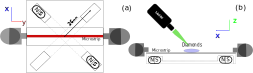
\includegraphics[width=0.7\linewidth]{../figures/magnets}
	\caption[Positioning of the magnets]{Positioning of the magnets exemplarily for one direction. Top and side view of the magnet positions}
	\label{fig:magnets}
\end{figure}


\subsection{Calibration}

\subsubsection{CCD Conversion Factor}
\label{sec:sizecal}

The length of the strip was measured with a calliper at $1.2\pm 0.1\mathrm{mm}$ and the camera used was a Thorlabs CCD camera had dimensions of 1280x1024 pixels, each pixel with $5.2\times5.2\,\mathrm{\mu m}$ according to the manufacturer.
In order to know the actual resolution of our microscope a calibration was done based on the magnification and calibration factor of the set up.
Theoretically our $C_{f}$ can be calculated from the lenses $f_{1}$ and $f_{2}$ that gives a Magnification of 8. The calibration factor is given by:
\\

\begin{equation}
C_{f}=\dfrac{1\,\mathrm{px} \cdot M}{d_{p}} = 1552\,\mathrm{px/mm,}
\end{equation}\\

where $M$ is the magnification and $d_{p}$ the pixel size.\\

For getting an experimental magnification we measure the distance in pixel of the microstrip using the the tool of Thorlab’s software and overlapping two pictures as shown in fig \ref{fig:distance-sslip}. The strip had in total 1442 pixels of cross section  with leads to  a magnification factor close to $M=7$.
Using the equation above and the respective measurement we denote that the conversion factor is measured to be $C_{f} =1346\pm224 \,\mathrm{px/mm}$ which will be used in section \ref{sec:size} to measure the size of the used diamond.

 \begin{figure}
 	\centering
 	\includegraphics[width=0.7\linewidth]{"../figures/distance sslip"}
 	\caption[Width of the microstrip]{Overlay of the two pictures that shows the width of the strip using a bright diamond in the centre as a reference point. The measurements was done in situ but the  image overlay was done with FIJI software in a post analysis.}
 	\label{fig:distance-sslip}
 \end{figure}
 

\subsubsection{Laser Power}
To set the power of the laser to a reasonable value a calibration curve was recorded which shows the actual laser power at the position of the Ms plotted over the output power set in the GUI. This curve is shown in figure \ref{fig:power}.\\

Using this graph the output power was set to $P_\text{out}=20\,\mathrm{mW}$ which corresponds to an actual laser power of $P_\text{act}=(27.4\pm1.4)\,\mathrm{mW}$.
\begin{figure}
	\centering
	\includegraphics[width=0.65\textwidth]{../figures/powercal.png}
	\caption{Measurement of the laser power}
	\label{fig:power}
\end{figure}


\subsubsection{Electronic components}


In order to perform our ODMR measurements it is crucial to determine the amount of microwave power deployed into the microstrip and the diamonds. We can not know the absolute power that is plugged in. The micro strip by default has some transmission $T_{Ms}$ and reflection $R_{Ms}$ that we need to measure experimentally.\\

For this, a power coupler is added to the set-up and four measurement with different configurations are performed as shown in figure \ref{fig:apd}. First, the power coupler (PC) is connected to the DSA to measure the out-in transmission $T_\text{out-in}$. On the other hand the second set-up, the in-cpl transmission of the Power Coupler $T_\text{in-cpl}$. Then the microstrip was connected to measure the transmission $T_\text{ms}^*$ and reflection $R_\text{ms}^*$ of the whole system consisting of the power coupler and the microstrip.


\begin{figure}[hb]
	\centering
	\includegraphics[width=0.7\linewidth]{../figures/APD}
	\caption[Measurements of the CPL and MicroStrip using the DSA]{Measurements of the CPL and MicroStrip using the DSA. (a) $T_\text{out-in}$ (b) $T_\text{in-cpl}$ (c) $R_\text{ms}^*$ (d) $T_\text{ms}^*$}
	\label{fig:apd}
\end{figure}

The SA was set at 0 dBm with a sweep centred at 2.8GHz frequency. A 50$\Omega$ resistance was used as an end resistor. The received signals are plotted in figure \ref{fig:microstrip}.\\

\begin{figure}
	\centering
	\includegraphics[width=0.7\linewidth]{../figures/microstrip}
	\caption[Microstrip Power Attenuation]{Attenuation of the power at 0dBm from top to bottom: $T_{CPL}$,$T_{Cpl-Ms}$, $R_{CPL}$ and $R_{Cpl-MS}$}
	\label{fig:microstrip}
	\end{figure}

The actual transmission and reflection of the microstrip was simply calculated by a subtraction of the microstrip transmission in the different processes using the following formulas:

\begin{align}
T_\text{ms}&=T_\text{ms}^*-T_\text{out-in}\\
R_\text{ms}&=R_\text{ms}^*+T_\text{out-in}-T_\text{in-cpl}
\end{align}


The calculated transmission and reflection is shown in figure \ref{fig:microstrip-trasm-eflect}. The attenuation for the transmission remains close to zero, specially in the centre of the sweep while the reflection as shown reduces drastic. This gives us the idea that the power transmitted is close to the 0dBm used in the SA and few of it is been reflected.

\begin{figure}
	\centering
	\includegraphics[width=0.7\linewidth]{../figures/microstrip-trasm-eflect}
	\caption[Microstrip transmission and reflection]{Attenuation of the resultant transmission (top) and reflection (bottom) at the Microstrip, at 0dBm in a 2.8GHZ frequency centre.}
	\label{fig:microstrip-trasm-eflect}
\end{figure}

\subsubsection{Optical Spectrometer}
The optical spectrometer is later used to record the fluorescence spectrum of the diamond. To calibrate the optical spectrometer we first record the spectrum of visible light and compare the identified Fraunhofer lines with their literature values. The recorded spectrum is shown in figure \ref{fig:sunspectrum} and the values are given in table \ref{tab:fraunhofer}.\\

Since only small statistical deviations in both directions could be found there was no need to calculate a conversion factor and the values given from the optical spectrometer were verified. \\

The optical spectrometer was also used to get the actual wavelength of the laser which was determined in figure \ref{fig:laserspectrum} to be $\lambda=(517.3\pm0.2)\,\mathrm{nm}$.
\begin{figure}
	\centering
	\includegraphics[width=0.8\textwidth]{../figures/sunspectrum.png}
	\caption[Spectrum of the sun with identified Fraunhofer lines]{Spectrum of the sun with identified Fraunhofer lines for calibration of the optical spectrometer}
	\label{fig:sunspectrum}
\end{figure}

\begin{table}
	\centering
	\begin{tabular}{c|c|c|c|c}
		Peak&Position&Element&Position \cite{fraunhoferlines}&Difference\\
		1&$526.8\pm1.7$&Fe I&527.0&$-0.2$\\
		2&$590.0\pm0.5$&Na I&589.6&$+0.4$\\
		3&$628.9\pm0.3$&Fe I&630.3&$-1.4$\\
		4&$657.2\pm0.3$&H $\alpha$&656.3&$+0.9$\\
		5&$688.6\pm0.5$&&&\\
		6&$763.5\pm1.3$&&&\\
		7&$824.7\pm0.3$&&&\\
	\end{tabular}
	\caption{Positions of the Fraunhofer Lines compared to the literature values}
	\label{tab:fraunhofer}
\end{table}

\begin{figure}
	\centering
	\includegraphics[width=0.8\textwidth]{../figures/laserspectrum.png}
	\caption[Spectrum of the laser]{Spectrum of the laser with identified peaks at the wavelengths $\lambda=(517.3\pm0.2)\,\mathrm{nm}$ and $\lambda=(1033.7\pm0.4)\,\mathrm{nm}$}
	\label{fig:laserspectrum}
\end{figure}

\subsubsection{ODMR calibrations}
\label{sec:odmr-cal}
\paragraph{Shielding}
To improve the ODMR signal and avoid noise generated by the microwaves a shielding cage was built around the APD. In figure \ref{fig:odmr-shield} the effect of this shielding cage on the ODMR spectrum is shown.
\begin{figure}
	\begin{subfigure}{0.5\textwidth}
		\includegraphics[width=\textwidth]{../figures/odmr-cal-1.png}
		\subcaption{without shielding}
	\end{subfigure}
	\begin{subfigure}{0.5\textwidth}	\includegraphics[width=\textwidth]{../figures/odmr-cal-2.png}
		\subcaption{with shielding}
	\end{subfigure}
	\caption{ODMR spectrum}
	\label{fig:odmr-shield}
\end{figure}
\paragraph{Time-to-Frequency Conversion}

\begin{figure}
	\begin{subfigure}{0.5\textwidth}
		\includegraphics[width=\textwidth]{../figures/odmr-cal-4.png}
		\subcaption{shifted to the left}
	\end{subfigure}
	\begin{subfigure}{0.5\textwidth}
		\includegraphics[width=\textwidth]{../figures/odmr-cal-3.png}
		\subcaption{shifted to the right}
	\end{subfigure}
	\caption{ODMR spectrum for time-to-frequency calibration}
	\label{fig:odmr-shift}
\end{figure}

Performing ODMR measurements we achieve the ODMR spectra on the oscilloscope. Therefore the spectra are time-resolved. To gain frequency-resolved spectra we need to calculate the conversion factor from time to frequency. We do this by performing two sweeps with shifted centre frequencies which allows us to calculate the conversion factor and also the offset since we know the frequency at which the peak appears.

The conversion can be expressed by the following equation:

\begin{align}
f(t)&=\frac{f(t_1)(t_1-t_2)-(f(t_1)-f(t_2))t_1}{t_1-t_2}+\frac{f(t_1)-f(t_2)}{t_1-t_2}\cdot t
\end{align}

Inserting the values achieved from figure \ref{fig:odmr-shift} we get the following conversion function:

\begin{align}
f(t)&=(1.003\pm0.003)\,\mathrm{\frac{GHz}{s}}\cdot t+(2.728\pm0.011)\,\mathrm{GHz}
\end{align}

Later in this document all spectra are converted by this function and therefore shown in the frequency domain. The errors are gained from the fit and propagated using Gaussian error propagation.

\subsection{Measurements}
\label{sec:measurements}
After the calibration measurements are finished the actual measurements will be started. First we measure the size of the diamond which is done with taking a picture of the diamond using the CCD and then measuring the distance using our conversion factor calculated in section \ref{sec:sizecal}.\\

Then we will take the fluorescence spectrum of the diamond using the optical spectrum analyser and look for the zero-phonon-line to make sure we have NV$^-$ centres inside the diamond.\\

The main part of our measurements will be the ODMR measurements. We will use the measurement technique described in section \ref{sec:odmr} which we already used in section \ref{sec:odmr-cal} and record an ODMR spectrum of the diamond. Afterwards we will turn on magnetic fields separately in $x$, $y$ and $z$ direction and measure the ODMR spectra for each magnetic field.